%# Database File : DTX-Geometria-EmbadaBasSxPythTheor-CombEx1
%@ Database source: Mathematics
\wrapr{-5mm}{10}{3.9cm}{-7mm}{
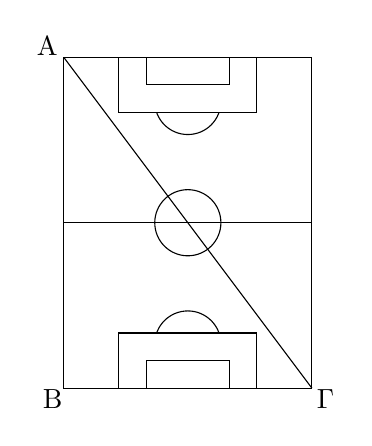
\begin{tikzpicture}[scale=.7]
\draw  (-4,4) rectangle (0.5,-2);
\draw (-4,1) -- (0.5,1);
\draw  (-1.75,3.2) ellipse (0.6 and 0.6);
\draw[fill=white]  (-3,4) rectangle (-0.5,3);
\draw[fill=white]  (-2.5,4) rectangle (-1,3.5);
\draw  (-1.75,-1.2) ellipse (0.6 and 0.6);
\draw[fill=white]   (-3,-2) rectangle (-0.5,-1);
\draw[fill=white]   (-2.5,-2) rectangle (-1,-1.5);
\draw  (-1.75,1) ellipse (0.6 and 0.6);
\node at (-4.3,4.2){A};
\node at (-4.2,-2.2) {B};
\node at (0.75,-2.2) {$\Gamma$};
\draw (-4,4) -- (0.5,-2);
\end{tikzpicture}}{
Το στάδιο Camp Nou βρίσκεται στην πόλη της Βαρκελώνης στην Ισπανία και είναι έδρα της ποδοσφαιρικής ομάδας FC Barcelona. Το μήκος $ AB $ του ποδοσφαιρικού γηπέδου είναι $ 105m $. Δίνεται γνωστό ότι η διαγώνια απόσταση $ A\varGamma $ ανάμεσα σε δύο απέναντι corner είναι $ 125{,}1m $.
\begin{rlist}
\item Πόσο είναι το πλάτος $ B\varGamma $ του γηπέδου;
\item Να βρεθεί το εμβαδόν που καταλαμβάνει η επιφάνεια του γηπέδου.
\item Αν γνωρίζουμε ότι το κόστος τοποθέτησης του χλοοτάπητα είναι 12\officialeuro\, για κάθε τ.μ. να βρεθεί το συνολικό κόστος τοποθέτησής του.
\end{rlist}}
%# End of file DTX-Geometria-EmbadaBasSxPythTheor-CombEx1